This subsection specifies the implementation details of the User Interface,
and should be considered together with figure \ref{fig:UI_views},
which illustrates the design proposed for the application.
The User Interface consists in a single page application,
divided into three main views: the \textit{Request}, \textit{Response} and \textit{Map view}.
Due to the implementation using React, every view is managed by a container,
which reads the state from the store, calls the rendering of presentational components,
and may dispatch actions on user input or other events. 

The User Interface is designed to be mobile friendly, by being responsive to the 
device size. This is achieved using the Bootstrap grid system, 
a website design paradigm in which the user screen is divided into 12 columns,
and each block of the user interface may specify a variable number of columns, depending on the screen size.

Figure \ref{fig:desktop_app} and \ref{fig:mobile_app} show the current versions of the developed applications.
The first image illustrates the application in a desktop device and the second in a mobile.
It is worth noting that these two screenshots correspond to the same application,
and that the design differences between both images are a result of the responsiveness of the application.
The responsive design is responsible for resizing the application elements according to the device size.
This responsiveness also includes toggles in the \textit{Request} and \textit{Response} views, as to generate more space 
to the map view. If this was not the case, it would become impossible to view the map in the mobile version.  


\begin{figure}[htpb]
  \centering
  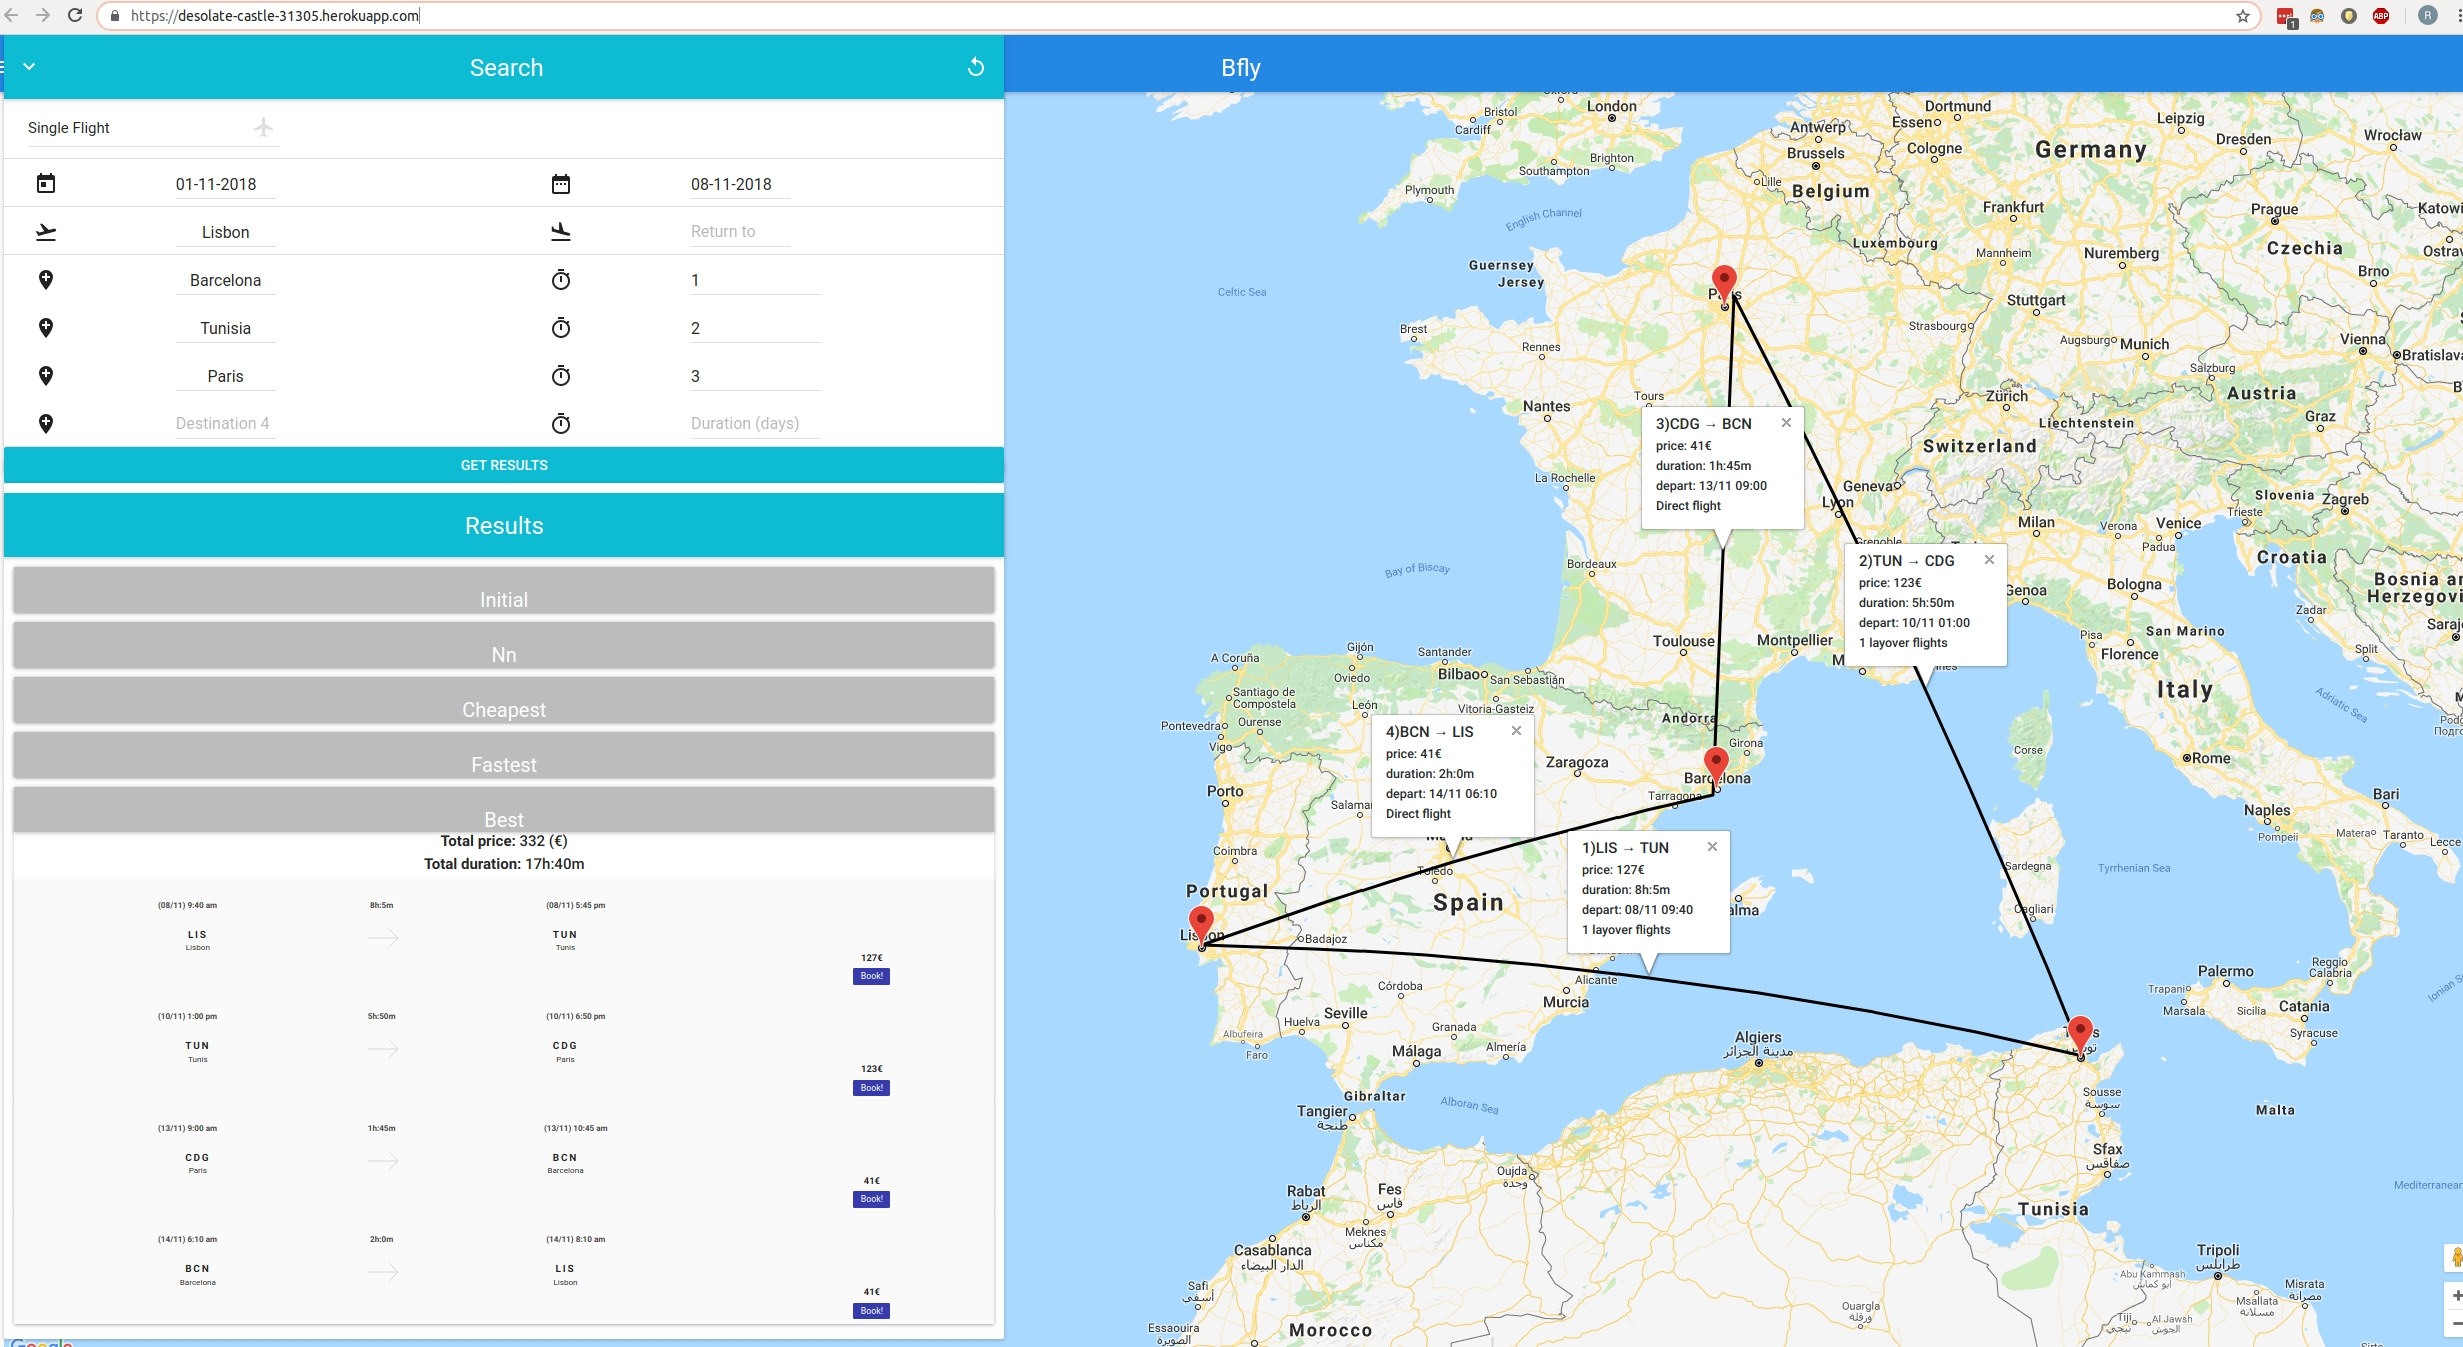
\includegraphics[width=\textwidth]{./imgs/bfly_desktop.jpg}
  \caption{Screenshot of the developed application rendered in a desktop device.}
  \label{fig:desktop_app}  
\end{figure}

\begin{figure}[htpb]
  \centering
  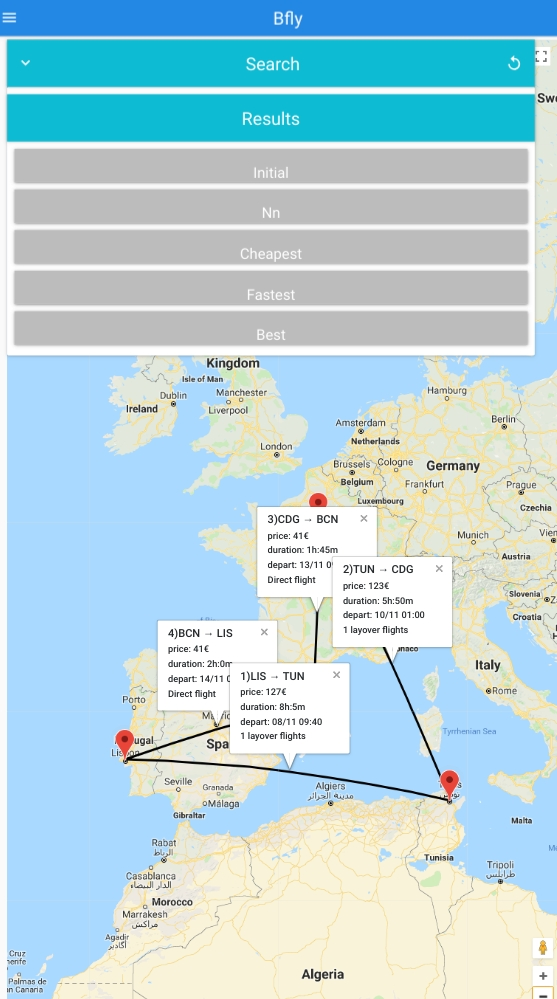
\includegraphics[width=\textwidth]{./imgs/bfly_mobile.jpg}
  \caption{Screenshot of the developed application rendered in a mobile device.}
  \label{fig:mobile_app}  
\end{figure}